\documentclass[10pt]{article}

\usepackage[margin=1in]{geometry}
\usepackage{amsmath,amsthm,amssymb}
\usepackage{graphicx}
\usepackage{subfig}
\usepackage{float}
\usepackage{wrapfig}
\usepackage{multicol}
 \usepackage{booktabs}
 \usepackage{hyperref}
 \hypersetup{
 	colorlinks=true,
 	linkcolor=blue,
 	filecolor=magenta,      
 	urlcolor=cyan,
 }

\graphicspath{ {/Users/clay/Documents/research/TGE-SP21/assignments/images/} }

\begin{document}

% --------------------------------------------------------------
%                         Start here
% --------------------------------------------------------------

\title{Assignment 2}%replace X with the appropriate number
\author{Geosc 597-003\\
Techniques of Geophysical Experimentation} %if necessary, replace with your course title

\maketitle

%\textit{\textbf{Objective(s):}
%Build on in-class blinking an LED (diode).}

\section*{Activity 1 - DCDT Calibration}

This is a follow-up to the calibrations that were carried out in the Rock Mechanics Lab on 27 Jan. Please work with your group members to determine an appropriate calibration for your particular DCDT/gain. You will find the raw data on the course GitHub repo under resources (will be uploaded on 4 or 5 Feb). \\ 
Please consider relevant aspects for sensors, such as linearity, etc. \\

\noindent\textbf{\textit{Do the following:}}
\begin{enumerate}
		\item Plot the raw data with a fitted line.
		\item Report the \textbf{slope} (absolute value) in \textbf{appropriate units} (mm/V) and $ R^2 $.
		\item Compare this calibration value to previous (see .xlsx sheet in resources directory in the github repo) -- how much has it changed? Is this reasonable, why? Referring back to the Lecture 2 slide deck may jog your memory.
\end{enumerate}

\begin{table}[h!]
	\footnotesize
	\centering
	\begin{tabular}{@{}ll@{}}
		\multicolumn{2}{c}{\textbf{Grading Rubric}} \\ \midrule 
		\multicolumn{1}{l}{\textit{Problem}}   & \textit{Points}   \\ \midrule 
		\#1                    & 5       \\ \midrule
		\#2            & 5       \\ \midrule
		\#3            & 15       \\ \midrule
		Total                            & 25       \\ \bottomrule
	\end{tabular}
\end{table}

 \clearpage
 
 
 
\section*{Activity 2 -  Voltage Divider Adventures}

In this activity you will apply our knowledge about circuits and voltage dividers. \\

\begin{figure}[ht]
	\centering
	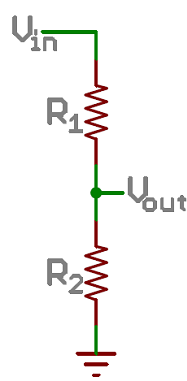
\includegraphics[width=0.1\columnwidth]{voltage_divider}
	\caption{Voltage divider circuit diagram.}
	\label{fig:stoplight_wiring_diagram}
	
\end{figure}

\noindent\textbf{\textit{Do the following:}}
\begin{enumerate}
	\item Set $ V_{in} $ as 5V and use 2 resistor of equal values. Plug $ V_{out} $ in this diagram into A0 on your Arduino and use the serial plotter.
	\begin{enumerate}
		\item Verify that your output at $ V_{out} $ is what you expected it to be -- recall the equation for a voltage divider. 
	\end{enumerate}
	\item Now set up your potentiometer as R1 and remove R2 in this diagram. Use the serial plotter to look at the output as you adjust the potentiometer. Is this what you expected?
	\item We should be used to seeing the voltage output of the potentiometer, so let's use it to control something physical. Control the brighness of a LED. 
	\begin{enumerate}
		\item Use what we've learned about circuits to explain how this setup works. 
	\end{enumerate}
\end{enumerate}

\begin{table}[h!]
	\footnotesize
	\centering
	\begin{tabular}{@{}ll@{}}
		\multicolumn{2}{c}{\textbf{Grading Rubric}} \\ \midrule 
		\multicolumn{1}{l}{\textit{Problem}}   & \textit{Points}   \\ \midrule 
		\#1                    & 20       \\ \midrule
		\#2            & 25       \\ \midrule
		\#3            & 30       \\ \midrule
		Total                            & 75       \\ \bottomrule
	\end{tabular}
\end{table}


\section*{What to upload to Canvas}
You should upload the following with \textit{consistent file names}:

\begin{itemize}
	\item Your Arduino codes. Make sure it works before you upload.
	\begin{itemize}
		\item \textbf{Fully comment your code!} The blinky example from the Arduino IDE is commented so that others can read the code and understands what is executed. 
		\item \textbf{Naming convention:} username\_blinky2.ino and username\_stoplight.ino\\
		Example: cew52\_blinky2.ino, cew52\_stoplight.ino.
		\item Put all Arduino codes for this assignment in a project folder. 
	\end{itemize}

	\item A short movie demonstrating the operation of adjusting LED brightness.
	\begin{itemize}
		\item \textbf{Naming convention:} username\_LED\_bright.mov
	\end{itemize}

	\item Put all files inside of a directory named: username\_assignment2
\end{itemize}

%\vspace{2cm}



\end{document}